

In this chapter, the background of data clumps will be discussed. A formal definition of code smells is given in \ref{sec:code_smell}. Then, section \ref{sec:data_clump_def} focues on a formal definition of data clumps and their refactoring while also outlining the challenges of this task.

The concept of Large Language Models are discussed in section \ref{sec:chatgpt}. Here, the potentials but als o the challenges of these models are outlined providing an overview of what a practitioner must be aware of.

In the end, related tools and related research will be discussed in section \ref{sec:related_research}. 




\section{Code smells}\label{sec:code_smell}

The term \enquote{Code smell} is suggested by Kent Beck in \cite{fowler2019refactoring} for source code that is functionally correct but hard to read or difficult to improve which can be an issue in the future. Removing those code smells is called refactoring. If the refactoring is not performed on time, the costs of maintenance of the source code and the software project can be higher, and the efficiency of implementing changes is reduced. Some examples of code smells include unclear variable names, large classes, over-sized methods, missing documentation, or code duplicates. 

Depending on how they affect maintenance  different type of code smell exists. For instance, \enquote{bloaters} are code smells that increases the code size unnecessarily. \enquote{Change preventers} are code smells where a small change in the source code necessitates additional changes in numerous other places to maintain functionality. \cite{data_clumps_refactoring_guru}


Another distinction of code smells is how easier they can be detected. Localized code smells can be spotted by analyzing a small amount of code lines (i.~e. it not essential to analyze multiple files to be sure of the existence of a code smell). Long parameter list or missing documentation is one example of local code smells.  In contrast, scattered code smells can only be detected by comparing multiple parts of the source code to each other (e.~g. strong coupling between classes). \cite{10.1007/978-3-030-29238-6_19}

In all these cases, the short term effects of refactoring are small to non-existent. For instance, the performance or bug resiliency of a program is not improved. In longer terms however, as the software must be adapted for future challenges, the advantages of refactoring become clear as the costs of finding and fixing bugs and implementing new features is reduced. 

One issue with regard to refactoring is code smell prioritization and filtering. Not all code smells are equally problematic and many developers disagree on what constitutes a code smell. Additionally,  the amount of resources to refactor code smells is correlated to the amount of code smells. \cite{10.1007/978-981-13-8300-7_21}

Therefore, the goal of refactoring is often not to eliminate all code smells at once but a subset of them that are deemed \enquote{important}. Determining and refactoring these code smells is an essential method to maximize the quality of the source code  given limited resources. \cite{code_smell_prio} 
\section{Data clumps}

This section changes the focus from code smells in general to data clumps. 

Firstly, an informal definition is presented in section \ref{sec:data_clump_def} which is contrasted to a formal definition that will be used in this master thesis. Additionally, important terms and concepts related to data clumps are discussed. 

Afterwards, the challenges of detecting a data clump are outlined in section \ref{sec:data_clump_detection}. 
Detecting data clumps does not remove them. Hence, section \ref{sec:data_clump_refactor} provides an overview about the methods that remove a data clump. 

However, not every data clump should be removed as there can be several arguments against such an action. These arguments are discussed in section \ref{sec:data_clump_not_refactor}.

Finally, it is important to represent data clumps in a format that allows other tools to work with them so that they can be analyzed and eventually refactored. Section \ref{sec:data_clump_graph} provides an overview over different strategies. 


\subsection{Data clump definition}\label{sec:data_clump_def}
The term \enquote{data clump} was coined by Martin Fowler as one possible code smell. 
Martin Fowler originally describes data clumps as follows:

\begin{displayquote}
\enquote{Data items tend to be like children: They enjoy hanging around together. Often you'll see
the same three or four data items together in lots of
places: as fields in a couple of classes, as parameters in many
method signatures. Bunches of data that hang around together really ought to find a home together.} \cite{fowler2019refactoring} 
\end{displayquote}


This definition is somewhat imprecise. It is not specified whether three or four data items are necessary. Also, \enquote{a couple of classes} and \enquote{in many method signatures} do not define concrete numbers. To help practitioners,   author suggests checking whether the removal of one data clump item would have a significant effect on the coherence of the code.

A more precise and algorithmic definition of \enquote{data clumps} is provided by Zhang et Al. in  \cite{zhangImprovingPrecisionFowler2008}. They say a data clump can be defined on the field or method-parameter levels. 
To be a method parameter data clump, a group of at least four parameters must appear in multiple methods. Those variables must be duplicated, meaning they share the same name and data type. However, the inner order of the group does not need to be the same. In this master thesis, these data clumps are referred to as \textbf{parameters-to-parameters data clumps}.

For field data clumps, similar conditions apply. There must be at least four fields that appear in more than one class, and the names and data types of the variables must be the same, while the inner order may be different. Since in most programming languages, a field can have an additional access modifier (e.g., \textit{private}, \textit{static} etc. ), the access modifier should also be included to determine whether two groups of variables are identical and hence a data clump.  Data clumps related to fields of different classes will be referred to as \textbf{fields-to-fields data clumps}.

Additionally, data clumps can also exist between a method and a class. if at least four fields of a class are similar to the parameters of a method, it can be considered as a data clump. However, it should be noted that based on this definition constructors or similar initialization methods can easily be flagged as data clumps because they require similar parameters to existing fields. Refactoring these can be deemed unnecessary as this repetition cannot be avoided. 
 In the following, these data clumps are referred to as \textbf{parameters-to-fields data clumps}


The criteria for determining whether a data clumps exists often needs to be more relaxed. For instance, methods can be inherited and overridden so that a group of parameters may appear in each derived class, thereby fulfilling the definition of a  parameters-to-parameters data clump. Since (except for the identifiers of the parameters) an overriding method must be the same as the overridden method, they are not considered data clumps.


Another relaxation worthy to consider is with respect to the type equality. If variable \textit{A} has the data type \textit{double} and variable \textit{B} has the type \textit{int}, any value in \textit{B} can be assigned to \textit{A} because no information is lost. Vice versa, this conversion can lead to information loss. As a result, there is a directed compatibility between \textit{A} and \textit{B}. Hence, it can be argued that both variables might be part of a data clump even though their data type is different. 


Also, modification of a variable's identifier might not change its meaning. For instance, typos can happen, or synonyms can be used so that an automatic algorithm might not discover the connection between two variables because it has no knowledge of the semantics of the source code. \cite{zhangImprovingPrecisionFowler2008}


Data clumps can be classified as bloaters because they require a longer signature of a method or a larger class. Especially in the case of methods, one can also classify them as change preventers because if new parameters are added, many method signatures and their associated calls must be modified.

To conclude, the core definition of a data clump is clear. However, this definition still leaves out some edge cases that require a semantic understanding of the source code. 



In the following, the definition by \cite{zhangImprovingPrecisionFowler2008} will be used. However,  instead of requiring at least four parameters or fields for a data clump, at least three are required. The reasons for this change is that also Fowler believes that three variables can be sufficient for a data clump. Additionally due to the looser definition, a higher number of data clumps will be found in a software project which can help to better statistically analyze data clumps. In the end, these are subjective thresholds that are open for discussion. The thresholds for fields-to-fields, parameters-to-fields, and parameters-to-parameters data clumps should therefore be parameterized. 




Figure \ref{fig:company_bill_tax} depicts as an UML-diagram a parameters-to-parameters data clump. The class \textit{Company} has two methods dealing with financial payments. Both methods  have three parameters, namely an IBAN, a monetary amount, and a transaction date. While this example is comparably small, there could be more classes and methods in a real-world application that receives these three parameters to perform financial operations. As a result, changing the method signature can be time-consuming. For instance, adding a description to a transaction requires changing all affected method signatures and their associated calls. Also changing the data type of the monetary value (e.~g. to a custom Money class) requires similar changes. Additionally, the readability of these methods might be not ideal as a reader might not know what a \textit{IBAN} is or what currency \textit{amount} represents. These facts must be outlined in the documentation which therefore needs to be duplicated for each method. 
 
\subsection{Identifying data clumps}\label{sec:data_clump_detection}
In contrast to localized code smells like large methods or missing documentation, data clumps can be classified as a scattered code smell although they can be localized too. Considering only a small area of the source code is often not enough because they can be spread over multiple classes and methods. 

The difficulty of identifying data clumps, hence, can vary strongly dependent of how many files are affected by a data clump. If a data clump resides in only one file (e.~g. many methods in the same file share parameters), a trained eye can spot them and apply the necessary refactorings. This \textbf{manual approach} requires however that the developer is willing to spend time detecting data clumps and removing them. 


\begin{figure}[ht!]
\begin{lstlisting}[numbers=left]
    holders := all potential data clump holders 
            with at least three items inside the project
     For each (h1, h2) in holder with h1 != h2
        common := intersection(h1, h2)
        if common.size>=3:
            reportDataClump(h1, h2, common)
        

\end{lstlisting}
\caption{Algorithm for detecting data clumps}
\label{lst:data_clumps_algo}
\end{figure}






Listing \ref{lst:data_clumps_algo} shows how an algorithm to find data clumps could be designed. In the first step all data clump holders must be identified.
A data clump holder is a class that has at least 3 fields or a method that has at least 3 parameters.  Only methods and classes for which source code is available should be analyzed because refactoring would be impossible otherwise. In case of methods, overridden methods should only be refactored if their super methods also constitutes a data clump that can be refactored.  For instance, if a method overrides another method of which the source code is not available (external library), refactoring would be infeasible. 
It should be noted that other programming languages like C++ can have other data clump holder (e.~g. global variables in namespaces). 


Afterwards, all distinct tuples of data clump holders are compared. If two data clump holders share at least 3 fields/parameters, they form a data clump which can be reported. Determining common variables require comparing the identifiers and types of the variables and determining whether they are similar as specified in section \ref{sec:data_clump_def}. However, finding common parameters between two data clump holders is not trivial.  For instance, the algorithm does not specify how the identifiers of two data clump holders are compared (strict equality, synonyms). A similar issue arises with the types of the variables.  Two identical type identifiers might refer to different types if they are not fully qualified. Therefore, the type names must be qualified so that they can be compared. These details can be crucial for performance optimization and accuracy of its result. 



If a data clump is detected, it can be reported for further processing. For instance, a warning could be displayed in an \ac{IDE} or the detected data clumps can be refactored. Here also, the concrete implementation is dependent on how the data clumps will be processed later.

This algorithm has some drawbacks. It has a time complexity of $\Theta(n^2)$ where $n$ is the number of potential data clump holders. Therefore, analyzing  large projects can be time-consuming unless the set of potential data clump holders is reduced beforehand. Nevertheless, it accurately finds every data clump and is deterministic.

In contrast, probabilistic methods use an artificial intelligence like a large language model to detect data clumps. These are non-deterministic, and their reasoning are not always explainable. However,  these key differences help them to find data clumps that are difficult to find with the algorithmic approach. For instance, they can use synonyms for comparing variable names. 
  
\subsection{Refactoring data clumps}\label{sec:data_clump_refactor}

After establishing criteria for detecting data clumps, the issue remains on how to refactor them.

There are several approaches for refactoring data clumps. The general approach is always feasible and suggested by Fowler.
He outlines two  steps to refactor a data clump:

In the  \textbf{Extract-Class}-step, a class with fields for each data clump item is extracted. A class for this purpose might already exist so that it can be re-used.

In the second step, \textbf{Preserve Whole Object} or \textbf{Introduce Parameter Object} might be applied. This means that the method's signature is changed so that the extracted class replaces the data clump items, and all references to the method are changed accordingly.

Figure \ref{fig:company_bill_tax} shows this refactoring approach. The \ac{UML} class diagram shows a class \textit{Company} with three methods, each method having the same three parameters. This data clump can be removed by extracting a class (e.~g.~\textit{TransactionDetails})

If the extracted class already exists, it can be challenging to identify such a class. Given a current refactoring process (i.~e. a bot or human being is currently refactoring data clumps), two possibilities can occur. Either it was created during the ongoing refactoring process so that its location and name is known, or such knowledge is missing. The former case is easy to handle.  The latter variant occurs if the extracted class is created after the data clump is introduced but the data clump is not fixed immediately, or the extracted class already existed but for some reasons the data clump was introduced. In this case, a suitable extracted class must be identified which requires extensive knowledge of the source code.

Additionally, there could be classes that are a superset of the required fields to refactor the data clump. Suppose a data clump \textit{x}, \textit{y}, \textit{z} needs to be refactored. There could be a  class \textit{Vector4D} which has the fields  \textit{x}, \textit{y}, \textit{z}, \textit{w}. One might use the existing 4D vector class for this purpose by defaulting \textit{w} to zero. However, since 4D vectors serve different purposes than 3D vectors, it might be more appropriate to create a dedicated 3D vector class.


In the case of fields-to-fields data clump, introducing a common base class or interface could also help to solve the data clump issue. The new base class contains all data clump items as fields and is inherited by the two classes. Assuming only single inheritance hierarchies are supported, this does not work if at least one class already inherits from another class. In this case, using interfaces instead of classes can partially solve the data clump issue, but the data clump fields still need to be defined for each class. The \ac{UML} class diagram in figure \ref{fig:move_fields_up} shows how this works in practice. Here, two classes (\textit{Player} and \textit{NPC}) share the same three fields and do inherit the same class. By moving these fields to the base class, the data clump is removed. 

Another approach for refactoring data clumps is applicable to parameters-to-parameters data clumps in the same class. In this case, the parameters can be extracted to fields and removed from the method signatures. However, this exposes these fields to other unrelated methods in the class while at the same time the connection between the new fields and the methods that use them fades. Figure \ref{fig:params_to_fields} shows this approach. Here, different database related methods require certain parameters to work. Each time a method is called,  arguments must be provided for each of these parameters. In the refactored example, the values could be provided via a constructor at the instantiation of the class so that the parameter lists are much shorter. 




\begin{figure}
\centering
    \begin{subfigure}[t]{0.8\columnwidth}
    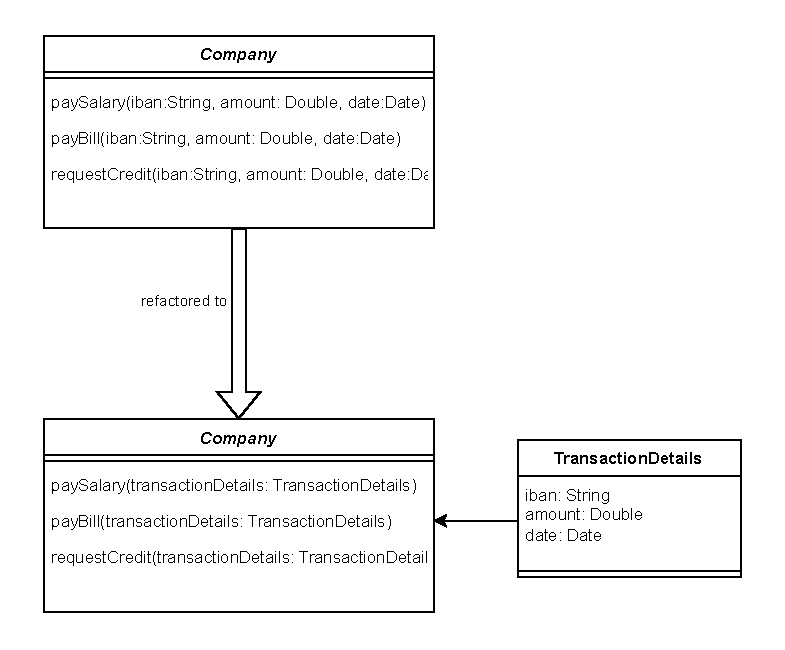
\includegraphics[width=1\columnwidth]{figures/chapter2/dataClump/refactor_simple_case.pdf}
    \caption{The standard approach by extracting a class}
    \label{fig:company_bill_tax}
    \end{subfigure}
       
    \begin{subfigure}[t]{0.4\columnwidth}
        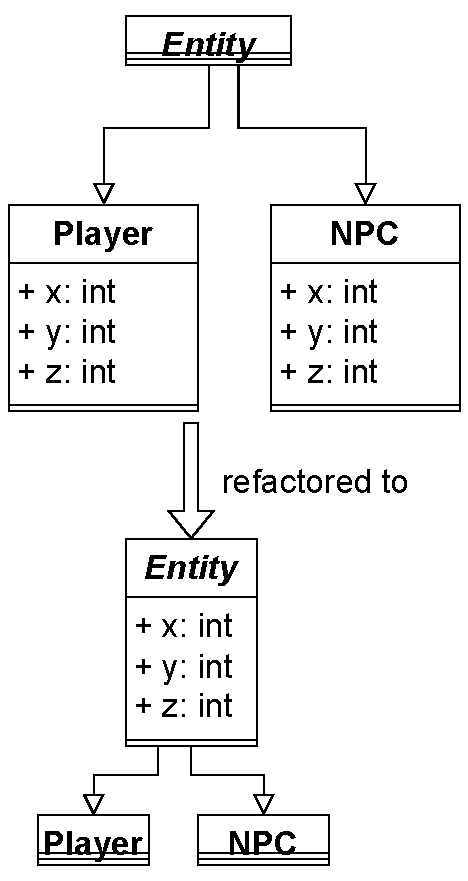
\includegraphics[width=1\columnwidth]{figures/chapter2/alternative_refactorings_move_up.drawio.pdf}
        
        \caption{By moving the fields to the base class}
        \label{fig:move_fields_up}
    \end{subfigure}
     \begin{subfigure}[t]{0.59\columnwidth}
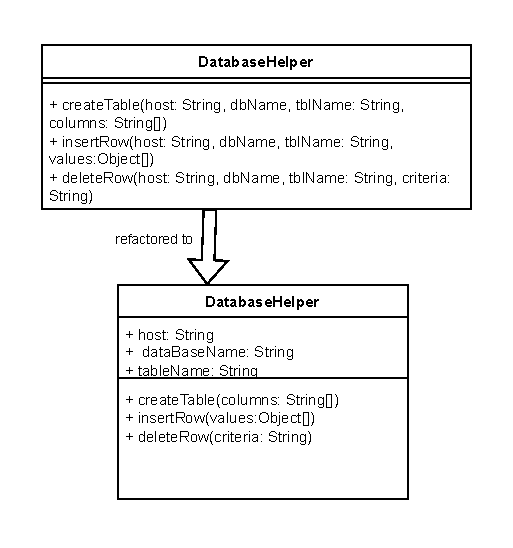
\includegraphics[width=1\columnwidth]{figures/chapter2/alternative_refactorings_to_fields.drawio.pdf}
\caption{By replacing parameters by fields}
\label{fig:params_to_fields}


    \end{subfigure}
\label{fig:refactoring_options}
\caption{Overview of refactoring options of data clumps}
\end{figure}


\subsection{Reasons not to refactor data clumps}\label{sec:data_clump_not_refactor}
As the previous section  outlines, each refactoring option has its drawback and might not be suitable in every circumstance.

Additionally, while data clumps can be classified as a code smell, there are situations where it would be considered not as a code smell or where refactoring is seen unnecessary. 

One reason for not refactoring data clumps is the tendency of producing data classes. These are classes that only provide access to data but no functionality. By extracting a class as outlined in section \ref{sec:data_clump_refactor} the new class has no or scarce additional functionality. These data classes can be also seen as a code smell so that refactoring might not reduce the number of code smells significantly. One way to mitigate this risk can be to further refactor the code by moving functionality related to the extracted class to such class thereby preventing data classes \cite{fowler2019refactoring}. 

Another problem is the creation of those extracted classes is object instantiation. Suppose a method previously requires three parameters \textit{x}, \textit{y}, and \textit{z}. For instance, consider a method that initially takes three parameters: \textit{x}, \textit{y}, and \textit{z}. After refactoring, this method would need just one parameter, an instance of the data class \textit{Point}, meaning callers must now create a \textit{Point} instance instead of providing three separate arguments. This could lead to the creation of many instances, consuming more memory and necessitating frequent garbage collection, thereby reducing performance. While these effects might be minimal, the effect is more significant on embedded systems or other systems with few resources. A similar problem occurs if the access to variables is replaced by getters or setters which also creates some overhead. While many compilers are capable of optimizing such issues, they should nevertheless be considered. 

Also over-engineering can be an issue. As noted in section \ref{sec:data_clump_def}, one can check the existence of a data clump by testing whether the removal of one parameter would make sense. This however is arbitrarily and no concise criteria can be given. Sometimes a group of parameters are connected but an extracted class would create a layer of abstraction that is unnecessary and makes the code even harder to read. This is particular important if the domain of each of the three variables is so distinctive that a common class name is hard to find. 
A popular paradigm in software development is \textit{Don't repeat yourself (DRY)} indicating that code duplication should usually be avoided and abstraction is preferred. However, the counter principle \textit{Write everything twice (WET)} has also gained attention as too much abstraction can hinder readability. \cite{dry}

In modular software projects, extracting a class can cause unwanted or even impossible dependencies.  Suppose a software project has a component for server-related code and for client-related code. Neither of this code is dependent of the other (i.~e. classes in one component are not visible in the other). A data clump connecting those components can only be refactored if the extracted class is located somewhere else. For instance, one could create a \textit{util} package. However, this creates an indirect dependency between server and client code and also might overload the \textit{util} package because it should not contain domain-specific code. 


\subsection{Representation of data clumps}\label{sec:data_clump_graph}

Data clumps can be represented as a graph, so that clusters or pattern can be detected to further evaluate whether a specific data clump is worth refactoring. 

For instance, a graph can be constructed that contains nodes for each class and additionally each method in the software project. If two methods form a data clump, they are connected by an edge in the graph representation. Similarly, two classes  are connected by an edge if there is a data clump relationship between the fields of these classes. 

Another approach is proposed by Baumgartner et al. Here, only the classes that contain data clumps are represented as nodes, and two nodes are connected by an edge if there is a data clump relationship between those two classes. For instance, an edge exists if a method in one class and another method in a separate class are part of a parameters-to-parameters data clump.~\cite{data_clumps_baumgartner}


One approach to represent and serialize data clumps for reporting purposes is the \textbf{Data clumps Type Context} \cite{dataclump_type_context} developed by Baumgartner et al. Each data clump is described by the affected files, classes and methods (if applicable). Additional, the precise location of each data clump is given. Hence,  it employs the first graph representation mentioned in this section, meaning that individual classes and methods are forming the data clump graph. However, the second variant can be re-constructed as well using this information. 
A full description of the format can be found in appendix~\ref{app:data_clump_format}.

To discern one data clump from another, a \textbf{types-names-identifier} is used in this master thesis. This identifier is created by sorting the data clump items by identifier, then joining the data type and identifier of each data clump with a white space, and concatenating these strings with a semicolon. For instance given a data clump \textit{boolean sign}, \textit{int exponent}, and \textit{double mantissa}. The respective types-names-identifier is \textit{int exponent;double mantissa;boolean sign}. This key identifies a data clump based on its types and names thereby helping to find related data clumps. 

The types-names id should be distinguished from the data clump id which uniquely identifies a given data clump. For instance, given a class with three methods (m1, m2, and m3) that share the same three parameters, there are three data clumps with three different ids (m1-m2, m1-m3, and m2-m3), but only one types-name-identifier as all methods share the same parameters. 

With this distinction, sub-problems of the refactoring process can be solved more easily. For instance, finding references of methods affected by a data clump requires that these methods are analyzed separately, therefore the unique id of each data clump must be used to separate the references. On the contrary, finding a suitable class name for a data clump is only dependent on the types and names of the data clump item so that the types-names id can be used. 






\section{Large Language Models}\label{sec:llm}

To successfully use an \ac{LLM}, it is essential to know how it operates and how it should be used correctly to improve the results. This section outlines the relevant background about \acp{LLM}. In the beginning, section \ref{sec:llm_introduction} outlines the technical background of \acp{LLM}. Afterwards, section  \ref{sec:chatgpt}  describes how ChatGPT can be used via the \ac{API} whose structure will be used as the foundation for a general \ac{LLM}-\ac{API} in later chapters. ChatGPT is contrasted to other alternative models in section \ref{sec:other_llm} highlighting that despite the popularity of ChatGPT, these options deserve consideration but have weaknesses too. In the remaining sections, weaknesses and advantages of \ac{LLM} in general are discussed. In section \ref{sec:llm_challenges}, the advantages and disadvantages of using \ac{LLM} are compared giving an overview of what arguments exist on both sides. The succeeding section \ref{sec:llm_considerations} discusses some problems that primarily arise if models are wrongly used and outlines how the quality of these models can be maximized. 


\subsection{Introduction}\label{sec:llm_introduction}
The term \ac{LLM} refers to a machine learning model that can generate and understand texts in an all-purpose manner. 

An \ac{LLM} is trained on a large data set of texts. These texts can come from books, internet pages or other textual sources. The input data is then prepared and sanitized to avoid biases and factual errors.


Then, the training process is performed. By word embedding, the relationship between words is trained such that the model learns the semantic relationship between words. For instance it can learn that cats are animals  or that there is a relationship between men and women. This relationship can be represented as vectors so that for example the relationship \enquote{men to women} can be applied to the term \enquote{king} which results in \enquote{queen}.

Which this training, the model is able to generate coherent texts based on an input that attempts to satisfy any query


For instance, given the text \enquote{How are}, the model  has a access to a corpus of texts where this sentence ends with \enquote{you} so that it is likely to finish the sentence with this word. 

To improve these results, fine tuning is performed. For instance, humans are asked to evaluate the outputs of a \ac{LLM} so eventual errors can be corrected or the model performs better for specific tasks.



Since source code can be viewed as a language, the methods can be applied too. However, specific fine-tuning is needed as source code  has a stricter syntax and a different data set(e.~g. public source code repositories).

It should be noted that a \ac{LLM} still has no sentience. Even if it seems to produce clear and meaningful output, it is still not aware of the inherent meaning. This can result in logical and confident output that is nevertheless wrong. \cite{Amaratunga2023}


\subsection{ChatGPT}
\label{sec:chatgpt}


ChatGPT \cite{ChatGPT_url} is a \ac{LLM} developed by OpenAI and released in November 2022. As a \ac{LLM}, ChatGPT can interpret user queries and return an appropriate response. 

A query can be a question or a prompt directing ChatGPT to answer a question or provide some output. The range of topics ChatGPT can help with is basically unlimited. For instance, ChatGPT can help with math, history, politics, or coding topics. ChatGPT can also understand programming language and therefore, help developers to code.  

The usage of ChatGPT is nevertheless somewhat restricted. For instance, content regarded as hate speech or used for illegal purposes will be suppressed.

Another essential feature of ChatGPT is the ability to store conversations. A conversation is a collection of queries and linked responses sent to ChatGPT. Using conversations, a user can refer to a previous query or response in a later query. For instance, if ChatGPT makes a mistake or misinterprets a query, a user can send another request connected to the previous request and point out the mistake or give more context, helping ChatGPT auto-correct itself. 

ChatGPT can be used via a browser or via an \ac{API}. Using ChatGPT via the browser is free, although restricted. A faster paid version is available and uses an improved model that supports larger ouputs and can process more data.

Figure \ref{fig:chatgpt_browser} illustrates how ChatGPT can be used in the browser.
\begin{figure}
    \centering
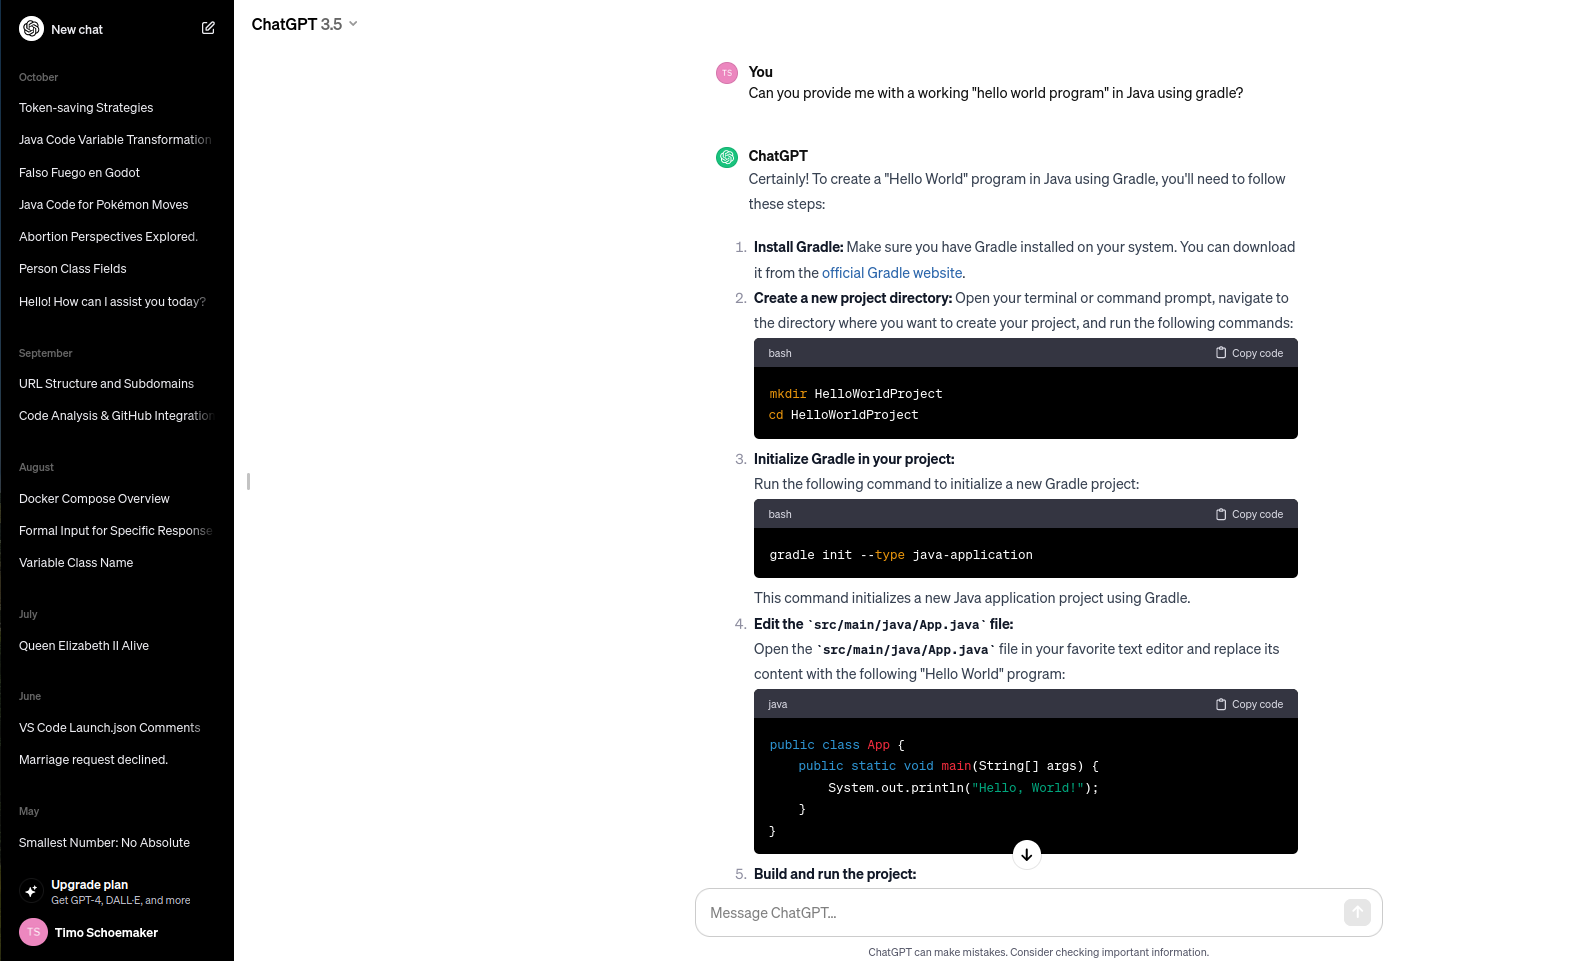
\includegraphics[width=\columnwidth]{figures/chapter2/chatgpt_browser.png}
    \caption{ChatGPT in the browser}
    \label{fig:chatgpt_browser}
\end{figure}
In the main panel that encompasses the most area of the figure, a chat is visualized. This is the the chat with the ChatGPT model. The queries are headlined with \textit{You} and the responses with \textit{ChatGPT}. In this example, ChatGPT is asked to create a \textit{hello world} program with gradle. As a response, the model returned code blocks that the user can simply copy and use. Also descriptions are provided to explain the context and usage of the code.

On the right side, all conversations with ChatGPT are listed. For instance, there is a conversation about \enquote{IntelliJ PSI Modification Fix}. A user can have multiple independent conversations where each has it own context. 

\subsubsection{API}
In order to utilize the ChatGPT \ac{API}, a user has to create an OpenAI account and provide financial information for billing purposes. Each request to the API consumes a certain amount of tokens dependent on the query. 

A token is the smallest unit used by ChatGPT to process a query. For instance, a token could be one English word, a syntactical part of a programming language, a number, or a similar discrete segment of a query. According to OpenAI, a token roughly equates 3/4 of a word, so 100 tokens are about 75 words. However, this is just an estimate for natural language texts in the English language. 

The \ac{API} itself used JSON combined with \ac{HTTP}. For the purpose of this master thesis, only a subset of the available means to use the \ac{API} will be explained because the whole \ac{API} would be too complex and outside the scope this master thesis. 

Listing \ref{lst:chatgpt_api} shows how an \ac{API} query may look like if it used via \textit{curl} which is a tool to  perform \ac{HTTP} requests:

 \begin{figure} [htbp!]
 \centering
			\scalebox{0.8}{\lstinputlisting
			[caption={ Example query to ChatGPT. based on  \cite{ChatGPT_url}}, 
			label={lst:chatgpt_api},
			captionpos=b,language=java, basicstyle=\footnotesize, tabsize=2, showstringspaces=false,  numbers=left]
			{figures/chapter2/chatgpt_api.json}}
		\end{figure}
 

Since ChatGPT uses \ac{JSON} for communication, the content header of \ac{HTTP}  must be set to \enquote{application/json} (l. 2). Subsequently, a token must be provided to ChatGPT (l. 23). which is generated on the OpenAI website and links the query to a specific OpenAI account for billing purposes. It is crucial that this token remains confidential and is not exposed (e.g., through version control systems).

Then, the actual query is defined (l. 4-24.). Firstly, the model is defined (l. 5). OpenAI provides multiple models that have different advantages and disadvantages. For instance, a newer model like \textit{gpt-4} has more capabilities but is more expensive.  By providing a temperature, a user can configure the randomness of the response (l.6). A higher temperature results in more creative answers but this creativity might worsen the quality of the responses. 

Afterward, the actual messages are provided (l. 7-25). Each message is a tuple of a \textbf{role} and a \textbf{content}. The content of a message is the input or output provided to or by ChatGPT. 

The role of a message indicates the source of a message. If the content of the messages comes from a user, the role should be \enquote{user} (l. 13). A reply for a query is defined as the role \enquote{assistant} (l. 17). The system role is a more specific and can be used to include further context for ChatGPT without eliciting a response (l. 9).

The response of the ChatGPT \ac{API} based on listing \ref{lst:chatgpt_api} is displayed in listing \ref{lst:chatgpt_api_response}.
 \begin{figure} [htbp!]
 \centering
			\scalebox{0.8}{\lstinputlisting
			[caption={The response from ChatGPT. Based on  \cite{ChatGPT_url}},
			label={lst:chatgpt_api_response},
			captionpos=b,language=java, basicstyle=\footnotesize, tabsize=2, showstringspaces=false,  numbers=left]
			{figures/chapter2/chatgpt_api_response.json}}
		\end{figure}

In the bottom part of the listing (l.~13-19), meta information is provided. This includes the response generation time (l.~12), the used model for the response (l.~14), and an id for the response (l.~13).

To enable clients to calculate the costs of using ChatGPT, each response also includes how many tokens have been used by the prompt (l.~18), by the response (l.~17), and the total number of tokens (l.~19).

In the upper part of the response (l. 1-11), the actual response is provided. The response is an array of so-called choices (l. 2~-~11). Each choice consists of the actual message (l.~ 6-8), which itself consists of the message content (l. 7) and the role of the content (usually \enquote{assistant}).

The \enquote{finish\_reason} indicates how the \ac{LLM} has finished on the prompt. If the value is \enquote{stop}, the prompt was executed without faults so that the response is valid. If the value is \enquote{length}, the output would exceed the maximum token limit, so the output will be incomplete. The value \enquote{content\_filter} indicates that OpenAI censured the requests because it violates the terms of use of OpenAI. \cite{ChatGPT_url}


\subsection{Other Large Language Models}\label{sec:other_llm}

While ChatGPT is the most known \ac{LLM}, there are several alternatives. This section gives only a broad overview as the focus will be on ChatGPT.

Some recent commercial \acp{LLM} services are Claude~\cite{claude} or Gemini~\cite{gemini}. Compared to ChatGPT, they differ in their training data, context window limitation, or maximum output size. Additionally, their pricing and API usage limits might be more favorable for some users.

A different method  is to use self-hosted \acp{LLM}.
Self-hosting means that the user of a \ac{LLM} has to provide for the infrastructure and resources to run and employ the model. For instance, a separate server could be configured that runs a large language model and listens to requests. This server could be directly set up by the user or rented from another organization (e.g virtual private server). 

With this approach, costs can be saved. Instead of being dependent on the price model of OpenAI which can be subject to changes, the user has to pay for the actual costs (e.g. the monthly rent for a server, the power bills, hardware etc). These might amortize after some years but this is not certain.

Moreover, privacy is more preserved since data does not flow to OpenAI but remains in the control of the user. This is especially important in regions with stricter privacy laws (e.~g. European Union).

A self-hosted \ac{LLM} is also more configurable. There a specific models that have been more intensively trained on coding tasks so that the quality of the results can be improved. The models from OpenAI are more generally trained.  For instance, the \textit{Llama2} model is specialized for human interaction while the \textit{Codellama} is specialized for discussing and generating source code. The \textit{Phind CodeLlama} model is based on the Codellama model and is focused more on the code generation task. 

However, this configuration requires effort and time. Finding a suitable model for a task, installing it, and configuring it is not trivial. For instance, a server needs to be set up that  runs the model, receives queries (e.~g. over a network) and respond back. 

This server must be suitable equipped. In general, at least 32 GB of RAM are necessary. Also video RAM and storage requirements must be met to gain useful performance. These are requirements that cannot be achieved by some users. 




Another problem with self-hosted \acp{LLM} is that they might have lower standards regarding output control. For instance, generating malicious or illegal content is easier with these models than those from OpenAI as they are more censored. 


Self-hosting \acfp{LLM} should not be confused with self-trained \acp{LLM}. In the latter case, a user must train its own model which requires extensive amount of data, even more processing power and the need to properly design the training process to prevent typical issues of machine learning like over-fitting.

\subsection{Advantages and challenges on using Large Language Models}\label{sec:llm_challenges}

While using  \ac{LLM} for refactoring brings many advantages  and possibilities, many challenges should be taken into account. The advantages and disadvantages will be discussed in this subsection. A \textbf{traditional approach} as used in this section means any manual refactoring algorithm (e.~g.,~ refactoring data clumps by extracting a class, removing and introducing parameters in methods, and updating all references)

\subsubsection{Advantages}

First of all, large language models are very flexible. A normal refactoring algorithm needs to consider many situations. For instance, a traditional approach that modifies the method signature in a class might not work on an interface. A large language model does not need to be adapted to all edge cases but often finds a suitable solution to a problem because it is not restricted to a specific refactoring process. \cite{shirafuji2023refactoring}

Additionally, a \ac{LLM} is more similar to a human as it is more  \enquote{creative}. While it is still a computer model and does not win the Turing-Test \cite{turing_test}, a \ac{LLM} can refactor code in a manner more closely as a human being would do. For instance, it can suggest class names that are related to the topic of the class, which a human being would also consider, while traditional approaches would use placeholder names, concatenation of field names or other simple name construction algorithms. \cite{shirafuji2023refactoring}

Large language models are also extensible. For instance, if another programming language is used, an \ac{LLM} can be easily adapted, while a traditional refactoring approach would require more effort to be language-agnostic.

Moreover, a \ac{LLM} can refactor the code in more ways than instructed. While a model can be specifically instructed to refactor data clumps, it might also correct formatting errors, spelling mistakes, or other code smells. While the focus of this master thesis will be on data clumps, other code smells are important too and might be more serious. Using a  \ac{LLM} allows developers to fix more code smells without developing and testing more tools to refactor multiple code smells. As they are better to understand the context of the code than a traditional approach, the quality of the code can therefore be improved. \cite{shirafuji2023refactoring}

Additionally,\acp{LLM} employ a interaction-based learning model which significantly facilitates the integration of developer feedback in real-time. This dynamic learning process allows \acp{LLM} to progressively refine and optimize their suggestions based on continuous interactions with developers. \cite{10.1145/3581641.3584037} 
%Furthermore, \ac{LLM} can adapt to the coding style of the source code. If for instance, the source code used the \enquote{snake\_case} or the \enquote{pascalCase} naming convention, the model can detect this convention and use it for its own refactoring (e.g. creating new methods, variables or classes). A traditional approach would need to be configured for each project to use the right convention so that the generated code might look more artificial as it does not not fit to the rest of the code.


\subsubsection{Disadvantages}

First of all \ac{LLM}s are not trustworthy. They are often confident in their answers which nevertheless are wrong. This confidence can often be broken by asking subsequent questions which lead the \ac{LLM} to rethink the answer. however, doing this in an automatic way is challenging. \cite{azaria2023internal}

Additionally, \ac{LLM} use randomness in their answers which means that the same query can result in different replies. The factors influencing the reply are generally not known and should not be assumed. As a result, requirements regarding a specific output format may be ignored by the model so that developers using a \ac{LLM} must always consider how to parse non-adhering output.  \cite{hu2023large}

One issue that many \acp{LLM} share is hallucination. This means that the model generates a response, but does not come to an end. For instance, an \ac{LLM} generating \ac{JSON} can add more and more \ac{JSON} objects to its response until it has no space left so that it must abruptly stop leaving an invalid \ac{JSON} with no closed braces.  The conditions when such behavior can be observed are unpredictable and should be taken care for. 

Furthermore, \ac{LLM}s are usually black boxes. They do not give hindsight on how they came to a specific reply. While they can explain their reasoning, it is not possible to check the exact thought process.
While a query can consist of multiple parts, conditions, or requirements, a \ac{LLM} will not always adhere to all of these. It may weigh some requirements, ignore other, or interpret them wrongly so that the result is unexpected. A \ac{LLM} may also come to an intermediate result that it will not show at the end even though the intermediate result was correct or requested. Also, no sources of the information is provided. \cite{chen2023instructzero}

Moreover, \ac{LLM}s do not have access to the latest information about a topic. They cannot access external sources like current news and up-to-date documentation. Instead, they employ a so-called cut-off date. Only information before that cut-off date will be used. As of the time of writing this section, the cut-off date for ChatGPT is April  2023. However, the release was several months later.  

There are also security issues with using  \ac{LLM} like ChatGPT. If a model is asked to generate or refactor code, one cannot trust that the code is safe to use. As a result of the cut-off date, the code might use operations that are considered deprecated or even unsafe to use because security vulnerabilities have been detected in the meantime. As a result, the developer needs to verify whether the code is safe to use which is another burden.  \cite{pearce2021asleep}

Furthermore, it is not out of the question that a malicious attacker might change the query or the reply of a \ac{LLM}. Therefore, using such a model might be a feasible way to hack systems or create damage which is difficult to detect and prevent. \cite{not_what_you_signed_for}

Another significant aspect are the legal implications of using \acp{LLM}. Since these models have only recently become mainstream, there are still unresolved legal issues. For instance, since most \acp{LLM} are trained using publicly available data, there are copyright issues as the idea of a particular line of code might come from somebody unknown. Also there are responsibility questions. What happens if the output of the model is malicious or faulty and who is legally responsible for making sure that no damage is done if the output of a model is used. The answers to these issues depend strongly on the jurisdiction. For instance, in the European Union the EU AI Act (Regulation (EU) 2024/1689), requires  transparency for using \acp{LLM} and bans the use of them in situation critical for human safety.  \cite{eu-ai-act}


Lastly, also costs and capacity considerations needs to be observed. For large projects, a \ac{LLM} might be too costly because  the costs are often dependent on the input size. Therefore, the use of large language models should be adequately prepared so that as much costs as possible can be saved.  \cite{chen2023frugalgpt}




\subsection{Consideration while using Large Language Models}\label{sec:llm_considerations}
In order to use a \ac{LLM} more effectively, many considerations should take place beforehand as the quality and potential costs can be strongly affected by them. While an \ac{LLM} can be very flexible and tolerant, ignoring these points nevertheless increases the risk of wrong results. These considerations are  referred to as \textbf{prompt engineering}. 

\subsubsection{Context window and statelessness}

Some \acp{LLM} (such as ChatGPT) are stateless.  This means that the server does not store conversations but delegates this task to the client.  This delegation becomes critical for prolonged interaction with a model. For instance, sometimes it desirable for a user to react to the output of a model by submitting feedback or query about topics that the initial reply does not cover. With a stateless \ac{LLM}, this second query can only be reasonably processed, if all previous messages such as the system message, the user messages, and the associated replies are again transmitted to the model. 


\begin{figure}
  \begin{adjustbox}{minipage=\linewidth,scale=0.7}
     \centering
     \begin{subfigure}[b]{0.3\textwidth}
         \centering
         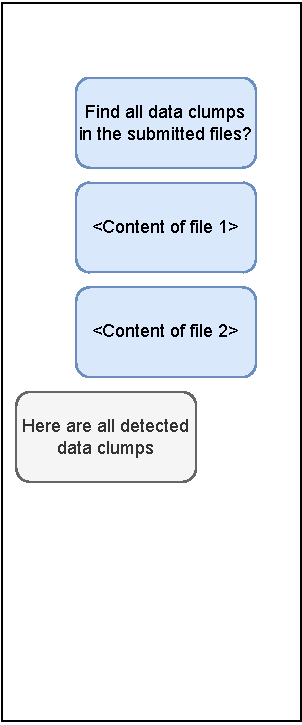
\includegraphics[width=\textwidth]{figures/chapter2/chatgpt_stateless_1.drawio.pdf}
         \caption{Initial request for data clumps}
        \label{fig:llm_stateless1}
     \end{subfigure}
     \hfill
     \begin{subfigure}[b]{0.30\textwidth}
         \centering
         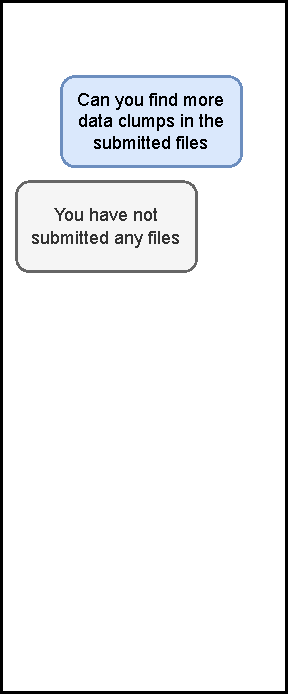
\includegraphics[width=\textwidth]{figures/chapter2/chatgpt_stateless_2.drawio.pdf}
         \caption{Second request without initial request}
         \label{fig:llm_stateless2}
     \end{subfigure}
     \hfill
     \begin{subfigure}[b]{0.3459\textwidth}
         \centering
         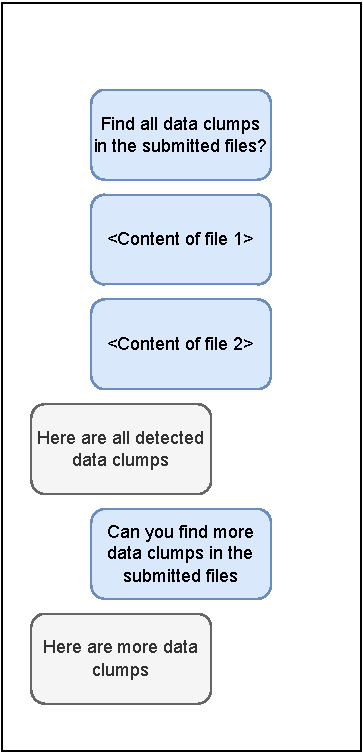
\includegraphics[width=\textwidth]{figures/chapter2/chatgpt_stateless_3.drawio.pdf}
 \caption{Second request with initial request}         \label{fig:llm_stateless3}
     \end{subfigure}
        \caption{Statelessness of \ac{LLM}}
        \label{fig:llm_stateless}
        \end{adjustbox}
\end{figure}

Figure \ref{fig:llm_stateless} visualizes this issue. The dialog with the model is represented as a chat similar to popular messaging programs. Each rectangle represents a distinct message. If it is left-aligned, the message originates from the model (output), otherwise it is a message provided by the user (input). 

In figure, \ref{fig:llm_stateless1}, the user asks a stateless model to find all data clumps in Java files. The \ac{LLM} responds with some data clumps. These might not be all data clumps, so a follow-up request might improve the results \cite{10062688}. Therefore, the user sends another completely new request in figure \ref{fig:llm_stateless2} to instruct the model to find more data clumps. However, the model responds with a general message stating that no files have been submitted. This is the result of the statelessness which requires that the user always send the whole context with each query. In figure \ref{fig:llm_stateless3}, the previous conversation history is provided so that the model accurately responds by finding another data clump.

For models that requires billing, this can be problematic  because the number of required tokens can enormously increase for longer conversations. However, even for self-hosted models, the initial request and the associated responses must be re-analyzed by the model which  consumes a significant amount of resources.


A related issue is the potential to forget information over longer conversations due to the context window. Large language models can only stores a limited amount of information during a conversation. If the amount of information is too large,  a model can react differently. ChatGPT will throw an error so that the user must reduce the amount of information transmitted to ChatGPT.

Other models will forget some parts of it even though they might be relevant for the use case of the \ac{LLM}. Figure \ref{fig:llm_loose_context} demonstrates the issues that arises.  A model is instructed to find and refactor data clumps in java files, and those java files are submitted as well. The response of the model at the bottom of the figure is however unexpected as it only explains the contents of the files submitted. The reason for this response is not some misunderstanding of the prompt but a lack of prompt. The transparent rectangle represents the context window, only covering the content of the transmitted files while the instruction is not covered. 
Because of the context window limitation, transmitting the third file overwrites the content of the prompt so that the model forgets the initial instruction and cannot reasonably process the files, giving instead a description of the files. The problem also arises on greater context window if multiple files or large files are involved as it may be the case while refactoring data clumps.

\begin{figure}[ht!]
    \centering
    \includesvg[width=0.6\columnwidth]{figures/chapter2/chatgpt_context_windows_size.drawio.svg}
    \caption{Example of model forgetting context}
    \label{fig:llm_loose_context}
\end{figure}

Also the output size of an \ac{LLM} is often limited. This means that generating larger text, the model might stop suddenly without finishing the text. In most cases, a \enquote{please continue} prompt can instruct the model to finish its response. The output limits are often reached when the model hallucinates. 
\subsubsection{Choosing the right parameters}
When dealing with an \ac{LLM}, a user must configure the model. The most major settings to be configured are the model itself and the temperature.

In this master thesis, the ChatGPT \ac{API} with the model \textit{gpt-4-1106-preview} is used as it provides a larger context  and output size and supports outputting in \ac{JSON} only. However, the cost associated with this model can be a disadvantage. Alternatively, the model \textit{gpt-3.5-turbo-1106} is cheaper but is not as thoroughly trained. For other providers of \acp{LLM}, other models are available that have their strengths and weaknesses.  

The temperature is another important configurable item. Using a higher temperature can be beneficial for creative tasks. On the other hand, the quality can be worse as the outputs can get more unpredictable. 




\subsubsection{Separate instruction and input}
Many queries to \ac{LLM} include an instruction and an input. For instance, a query to find and refactor data clumps could provide the source code containing the possible data clumps \textbf{(input)}. The instruction could be the query \enquote{Find and refactor all data clumps in this source code}. 

OpenAI recommends that the instructions and input be separated as distinctive as possible. It suggests enclosing the input in a block of \textit{"""} or \textit{\#\#\#} to mark what the input and what the instruction is clearly. For other models, other separation methods might work better as other training data was used but the general idea of this division is always beneficial. 

\subsubsection{Provide detailed context and how the model should respond}

When generating a reply to a query, a language model will use the available context to process the query and generate an output that attempts to satisfy the user's need. This means that every bit of relevant information can help the language model to generate a better response.

On the contrary, providing irrelevant information can increase the chance of wrong responses, so the creator of a query must always consider what to include in a query and what not. 

In the context of data clump refactoring, the query should include the content of the source code and the programming language. However, files that cannot have data clumps (e.g., configuration files) should not be included.

An instruction for refactoring data clumps should state that only the refactored source code files should be returned without providing explanatory texts or other information, as they can hinder the parsing of the output. 

Some models have the advantage of supporting specific output formats which eases parsing
For instance, when using the \enquote{gpt-4-1106-preview} or \enquote{gpt-3.5-turbo-1106} model of the OpenAI-\ac{API}, developers can force the model to respond in \ac{JSON}. Hence, the output can be made more predictable and easier to control. A request using this mode must include the term \enquote{\ac{JSON}}. It should however be noted, that the precise structure of the \ac{JSON} returned may still differ from the request. 


\subsubsection{Chain-of-Thought Prompting}\label{sec:chain of thought}

One way to improve the results from \acp{LLM} like ChatGPT is to separate a query into interconnected sub-queries that lead to a chain of thought. This can be compared to the human thinking process because a human alone tries not to solve a problem at once but breaks it down into simpler problems that are still inter-connected to but easier to solve. \cite{Wei2022ChainOT}

For instance, a query to find and refactor data clumps can be separated into a detection query and a refactoring query. These sub-queries can be further divided into a query for each file or for all files in a single directory. As a result, not one a single query is needed but multiple queries. 

This is useful if a human is reviewing the output from a \ac{LLM} since obvious errors can be spotted more easily if the task is divided into multiple steps. However, it is more challenging for an automated tool since it cannot find errors in the same way. 

Furthermore, one should consider that each queries requires further overhead so that the performance might be impacted more negatively. 





\begin{comment}
\subsubsection{Hosting a large language server}

One method to host a \ac{LLM} is via \textit{Ollama} \cite{ollama}. Ollama is a program to download, configure, and host a local \ac{LLM}. Users can set up a large language model with one command and query the model via the command line or a \ac{HTTP} interface.



After a model has been downloaded, a user can execute the command \textit{ollama run <model>} to submit queries 

Similar to to ChatGPT, there is an \ac{API} to integrate Ollama in other application. After installed, Ollama listens to \ac{HTTP} connections  on localhost and port 11434.

Listing \ref{lst:ollama_request} shows how such an \ac{API} can be used via \textit{curl}.

The difference to the ChatGPT \ac{API} are scarce. In contrast to ChatGPT, there is no header for an authorization token because no direct payment to any organization is needed. 

Additionally, Ollama streams replies by default meaning that not the full response is returned at once but multiple response parts that must be aggregated by the user. As this is not useful in the context of this master thesis, it is disabled by setting stream to false (l. 11).

Moreover, another model is used (l.~4) as the ChatGPT models are not available. 


 \begin{figure} [htbp!]. 
			\lstinputlisting
			[caption={ Example query to ChatGPT  \cite{ChatGPT_url}},
			label={lst:ollama_request},
			captionpos=b,language=json, basicstyle=\footnotesize, tabsize=2, showstringspaces=false,  numbers=left]
			{figures/chapter2/ollama/ollama_request}
		\end{figure}

  \end{comment}
\section{Related work}\label{sec:related_research}
The problem of data clump detection and refactoring is addressed in multiple papers. Also the  use of large language models in software development is a fairly recent rearch topic. In this section, research to both topics will be outlined: 

\subsection{Related to data clumps}
Baumgartner et al. developed a live code smell detection plugin for IntelliJ that can detect, report, and refactor data clumps without significantly impacting performance. However, the tool is semi-automatic, meaning the developer must still actively approve the data clump refactoring and suggest a suitable class name for the extracted class. \cite{BaumgartnerAP23}

As outlined in section \ref{sec:data_clump_def}, the definition of data clump by Fowler \cite{fowler2019refactoring} is somewhat ambiguous because no clear criteria to determine data clumps is established. Zang et al. \cite{zhangImprovingPrecisionFowler2008} creates a more algorithmic approach to determine whether a data clump exists. This approach is also explained in section \ref{sec:data_clump_def}. The authors also provide more precise definitions of other code smells like \enquote{message chains} or \enquote{speculative generality}. By interviewing four software development experts about the code smell definitions the authors developed, they find that their new data clump definition receives relatively more disagreement than other definitions, which the authors explain are the results of not covering edge cases in the definitions. 


Hall et al. analyzed the impact of code smells (including data clump) on the occurrence of faults in three open-source software projects. They find that data clumps have a mixed correlation to faults because, in two of the three projects analyzed, the correlation of data clumps per \ac{LOC} to detected faults is negative for two projects and positive for one project. This rejects their hypothesis that data clumps do not affect faults, and the authors suggest that the application domain and the development context need to be considered before the time-consuming refactoring of data clumps since their impact is not predictable.  \cite{hallCodeSmellsHave2014}


Murphy et al. \cite{stench_blossom} developed a visual tool to find code smells (including data clumps). the tool named \textit{Stench Blossom} is a plugin for Eclipse. If a plugin user views a file, the tool searches for code smells and displays them at the right side of the eclipse editor. Each code smell is visually displayed as a a \textbf{petal}. The radius of such petal represents the strength of a smell (i.~e. how strongly violates the code smell the given coding guidelines). The petal has a color that indicates how obvious a code smell is. Orange code smells are not very obvious while blue code smells are easy to detect by human beings. Since orange has a closer connection to warnings, it is more easily to perceive so that undetected code smells can be fixed better. Experiments with \textit{Stench Blossom} shows that the median number of code smells detected by humans using the tool increased from 11 to 21. However, data particular for data clumps is not given.  

\begin{comment}
Neto et al. developed an agent-based platform to detect and refactor code smells (including data clumps). The platform uses everal agents that work regularly to fix code smells. Each can obtain norms that describes what code smells it should fix, what conditions 
\end{comment}
\subsection{Related to large language models in software development}

White et al. \cite{White2023ChatGPTPP} outline how ChatGPT can be used in software development to improve the worklflow of developers. This includes  exploration of requirements, removing ambiguity in technical specification, or describing source code. The authors suggest specific prompts to elicit a suitable response from ChatGPt.

In case of refactoring, the author suggest that ChatGPT is able to refactor code with multiple prompts. For instance, ChatGPT can refactor based on a well known design pattern name, multiple examples on how to refactor the code, or a more lengthy requirements description. The exact success of each prompt is however dependent on how ChatGPT is trained and should be scrutinized manually. 

Cao et al. \cite{cao2023study} focus on using ChatGPT for fixing deep learning programs. Those are programs that cannot be understood only by their source code alone, but are are largely influenced by underlying data like  neural networks etc. This makes finding faults more difficult. The study finds out that ChatGPT can find code smells and detect faults. Without giving instructions however, ChatGPT will tend to return code smells and outdated API calls while not finding other bugs. 

\subsection{Refactoring tools}

\subsubsection{ Program Structure Interface}\label{sec:psi}
The Program Structure Interface provided by IntelliJ is an \ac{API} to analyze and modify  projects that the \ac{IDE} \textit{IntelliJ} can load. As a result, the various classes, methods etc. can be obtained which allows for the detection of data clumps. Also modifications are possible so that data clumps can be refactored.

In order to use this API, an instance of IntelliJ must be started. IntelliJ can be started in a headless mode to reduce loading times and improve the performance so that no GUI is initialized. Nevertheless, IntelliJ requires many resources and much overhead, so that  the initialization needs some time.

\begin{comment}
\section{Related work}
Since refactoring code smells is becoming increasingly important for developers, a variety of research has been conducted to study how the refactoring process can be improved.

Furthermore, tools have been developed that on their own cannot refactor code smells but can be adapted and used to ease developing refactoring tools.

Additionally, the use of \ac{LLM} in software development has recently gained widespread attention and has become a focus of several studies which analyzes the potential and challenges in practice. 

\subsection{Tools to assists data clump refactoring}





\end{comment}